%%%%%%%%%%%%%%%%%%%%%%%%%%%%%%%%%%%%%%%%%%%%%%%%%%%%%%%%%%%%%%%%%%
%
% Analysis of Algorithms
%
% Homework Assignment #3
%
%%%%%%%%%%%%%%%%%%%%%%%%%%%%%%%%%%%%%%%%%%%%%%%%%%%%%%%%%%%%%%%%%%
%%%%%%%%%%%%%%%%%%%%%%%%%%%%%%%%%%%%%%%%%%%%%%%%%%%%%%%%%%%%%%%%%%
%
% Score Card and Answer Sheets
%
%%%%%%%%%%%%%%%%%%%%%%%%%%%%%%%%%%%%%%%%%%%%%%%%%%%%%%%%%%%%%%%%%%
\documentclass[addpoints,11pt]{exam}
\usepackage{clrscode4e}
\usepackage{tcucosc}
\usepackage{units}
\usepackage{enumitem}
\usepackage{hyperref}
\usepackage{tikz}
\usetikzlibrary{trees}
%%%%%%%%%%%%%%%%%%%%%%%%%%%%%%%%%%%%%%%%%%%%%%%%%%%%%%%%%%%%%%%%%%
%
% Begin Document
%
%%%%%%%%%%%%%%%%%%%%%%%%%%%%%%%%%%%%%%%%%%%%%%%%%%%%%%%%%%%%%%%%%%
\begin{document}
	\pagestyle{empty}
	
	
	\noindent{\large\bfseries Name: Sabyasachi Sahoo}\\
	\noindent{\large\bfseries COSC 40403 - Analysis of Algorithms: Fall 2018: Homework 3}\\
	\noindent{\large\bfseries Due: 23:59:59 on September 18, 2018}
	
	%%%%%%%%%%%%%%%%%%%%%%%%%%%%%%%%%%%%%%%%%%%%%%%%%%%%%%%%%%%%%%%%%%
	%
	% Score Card and Answer Sheets
	%
	% Comment out one-or-the-other to show or not-show the answers.
	%
	%%%%%%%%%%%%%%%%%%%%%%%%%%%%%%%%%%%%%%%%%%%%%%%%%%%%%%%%%%%%%%%%%%
	\printanswers
	%\noprintanswers
	
	
	%%%%%%%%%%%%%%%%%%%%%%%%%%%%%%%%%%%%%%%%%%%%%%%%%%%%%%%%%%%%%%%%%%
	%
	% Score Card
	%
	%%%%%%%%%%%%%%%%%%%%%%%%%%%%%%%%%%%%%%%%%%%%%%%%%%%%%%%%%%%%%%%%%%
	\ifprintanswers
	\noindent
	\begin{center}
		\gradetable[v][questions]
	\end{center}
	\newpage
	\fi
	
	
	%%%%%%%%%%%%%%%%%%%%%%%%%%%%%%%%%%%%%%%%%%%%%%%%%%%%%%%%%%%%%%%%%%
	%
	% Question 1
	%
	%%%%%%%%%%%%%%%%%%%%%%%%%%%%%%%%%%%%%%%%%%%%%%%%%%%%%%%%%%%%%%%%%%
	\begin{questions}
		\question[5]
		6.1-1.  What are the minimum and maximum number of elements in a heap of height $h$?
		
		\begin{solutionorbox}
			Minimum: The minimum no. of nodes are when the last level has only one node i.e., $2^h$.\\
			Maximum: The maximum no. of nodes are when the last level is completely full i.e., $2^{h+1}-1$.
		\end{solutionorbox}
		
		\ifprintanswers
		\newpage
		\else
		\bigskip
		\fi
		
		
		%%%%%%%%%%%%%%%%%%%%%%%%%%%%%%%%%%%%%%%%%%%%%%%%%%%%%%%%%%%%%%%%%%
		%
		% Question 2
		%
		%%%%%%%%%%%%%%%%%%%%%%%%%%%%%%%%%%%%%%%%%%%%%%%%%%%%%%%%%%%%%%%%%%
		\question[5]
		6.1-2.  Show that an $n$-element heap has height $\floor{\lg n}$.
		
		\begin{solutionorbox}\\
			From Question-1 we get,\\
			an n-element heap must satisfy $2^h$ $\leq$ n $\leq$ $2^{h+1}-1$ $\leq$ $2^{h+1}$.\\
			Taking log on the sides we get, h $\leq$ lg n $\leq$ h+1.\\
			So, h = lgn + $\alpha$ \\
			where 0 $\leq$ $\alpha$ $<$ 1 \\
			Thus h = $\floor{lg n}$.
		\end{solutionorbox}
		\ifprintanswers
		\newpage
		\else
		\bigskip
		\fi
		
		
		%%%%%%%%%%%%%%%%%%%%%%%%%%%%%%%%%%%%%%%%%%%%%%%%%%%%%%%%%%%%%%%%%%
		%
		% Question 3
		%
		%%%%%%%%%%%%%%%%%%%%%%%%%%%%%%%%%%%%%%%%%%%%%%%%%%%%%%%%%%%%%%%%%%
		\question[5]
		6.1-6.  Is the array with values $\left<23, 17, 114, 6, 13, 10, 1, 5, 7, 12\right>$ a max-heap?  Show your work by using computer software to draw the heap.
		
		\begin{solutionorbox}
			\\
			\\
			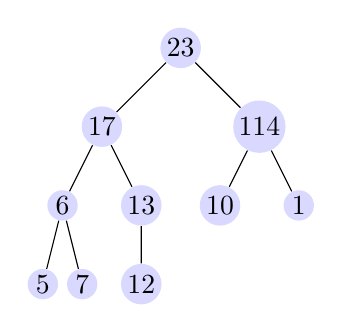
\begin{tikzpicture}[level distance=10mm] 
			\tikzstyle{every node}=[fill=blue!15,circle,inner sep=1pt] 
			\tikzstyle{level 1}=[sibling distance=20mm, 
			set style={{every node}+=[fill=blue!15]}] 
			\tikzstyle{level 2}=[sibling distance=10mm, 
			set style={{every node}+=[fill=blue!15]}] 
			\tikzstyle{level 3}=[sibling distance=5mm, 
			set style={{every node}+=[fill=blue!15]}] 
			\node {23} 
			child {node {17} 
				child {node {6} 
					child {node {5}} 
					child {node {7}} 
				} 
				child {node {13} 
					child {node {12}}
				} 
			} 
			child {node {114} 
				child {node {10}  
				} 
				child {node {1}} 
			}; 
			\end{tikzpicture}\\
			\\
			It is not a max-heap because (A,4) is not max-heapified as 6 $<$ 7.
			
		\end{solutionorbox}
		
		\ifprintanswers
		\newpage
		\else
		\bigskip
		\fi
		
		
		%%%%%%%%%%%%%%%%%%%%%%%%%%%%%%%%%%%%%%%%%%%%%%%%%%%%%%%%%%%%%%%%%%
		%
		% Question 4
		%
		%%%%%%%%%%%%%%%%%%%%%%%%%%%%%%%%%%%%%%%%%%%%%%%%%%%%%%%%%%%%%%%%%%
		\question[5]
		6.2-1.  Using Figure 6.2 as a model, illustrate (with computer software) the operation of $\proc{Max-Heapify}{(A,3)}$ on the array $A = \left< 27, 17, 3, 16, 13, 10, 1, 5, 7, 12, 4, 8, 9, 0\right>$.
		
		\begin{solutionorbox}
			\begin{enumerate}[label=(\roman*)]
				
				\item Step 1:
				
				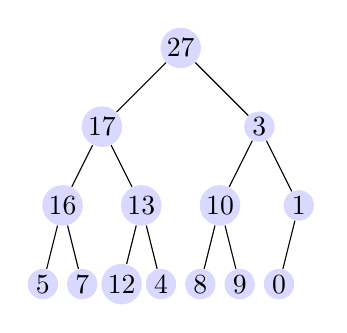
\begin{tikzpicture}[level distance=10mm] 
				\tikzstyle{every node}=[fill=blue!15,circle,inner sep=1pt] 
				\tikzstyle{level 1}=[sibling distance=20mm, 
				set style={{every node}+=[fill=blue!15]}] 
				\tikzstyle{level 2}=[sibling distance=10mm, 
				set style={{every node}+=[fill=blue!15]}] 
				\tikzstyle{level 3}=[sibling distance=5mm, 
				set style={{every node}+=[fill=blue!15]}] 
				\node {27} 
				child {node {17} 
					child {node {16} 
						child {node {5}} 
						child {node {7}} 
					} 
					child {node {13} 
						child {node {12}} 
						child {node {4}} 
					} 
				} 
				child {node {3} 
					child {node {10} 
						child {node {8}} 
						child {node {9}}	
					} 
					child {node {1}
						child {node {0}}
						child[fill=none] {edge from parent[draw=none]}
					}
				}; 
				\end{tikzpicture}
				
				\item Step 2:
				
				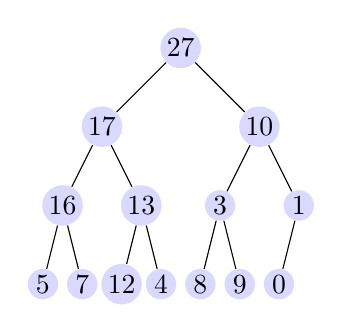
\begin{tikzpicture}[level distance=10mm] 
				\tikzstyle{every node}=[fill=blue!15,circle,inner sep=1pt] 
				\tikzstyle{level 1}=[sibling distance=20mm, 
				set style={{every node}+=[fill=blue!15]}] 
				\tikzstyle{level 2}=[sibling distance=10mm, 
				set style={{every node}+=[fill=blue!15]}] 
				\tikzstyle{level 3}=[sibling distance=5mm, 
				set style={{every node}+=[fill=blue!15]}] 
				\node {27} 
				child {node {17} 
					child {node {16} 
						child {node {5}} 
						child {node {7}} 
					} 
					child {node {13} 
						child {node {12}} 
						child {node {4}} 
					} 
				} 
				child {node {10} 
					child {node {3} 
						child {node {8}} 
						child {node {9}}	
					} 
					child {node {1}
						child {node {0}}
						child[fill=none] {edge from parent[draw=none]}
					}
				}; 
				\end{tikzpicture}
				
				\item Step 3:
				
				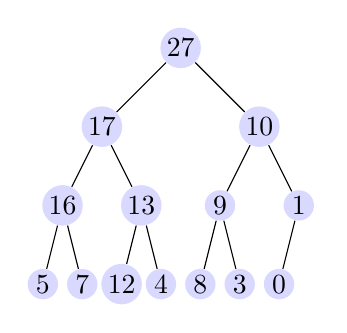
\begin{tikzpicture}[level distance=10mm] 
				\tikzstyle{every node}=[fill=blue!15,circle,inner sep=1pt] 
				\tikzstyle{level 1}=[sibling distance=20mm, 
				set style={{every node}+=[fill=blue!15]}] 
				\tikzstyle{level 2}=[sibling distance=10mm, 
				set style={{every node}+=[fill=blue!15]}] 
				\tikzstyle{level 3}=[sibling distance=5mm, 
				set style={{every node}+=[fill=blue!15]}] 
				\node {27} 
				child {node {17} 
					child {node {16} 
						child {node {5}} 
						child {node {7}} 
					} 
					child {node {13} 
						child {node {12}} 
						child {node {4}} 
					} 
				} 
				child {node {10} 
					child {node {9} 
						child {node {8}} 
						child {node {3}}	
					} 
					child {node {1}
						child {node {0}}
						child[fill=none] {edge from parent[draw=none]}
					}
				}; 
				\end{tikzpicture}
				
				
			\end{enumerate}
		\end{solutionorbox}
		
		\ifprintanswers
		\newpage
		\else
		\bigskip
		\fi
		
		
		%%%%%%%%%%%%%%%%%%%%%%%%%%%%%%%%%%%%%%%%%%%%%%%%%%%%%%%%%%%%%%%%%%
		%
		% Question 5
		%
		%%%%%%%%%%%%%%%%%%%%%%%%%%%%%%%%%%%%%%%%%%%%%%%%%%%%%%%%%%%%%%%%%%
		\question[5]
		6.2-2.  Starting with the procedure $\proc{Max-Heapify}{(A,i)}$, write pseudocode for the procedure $\proc{Min-Heapify}{(A,i)}$, which performs the corresponding manipulation on a min-heap.  How does the running time of $\proc{Min-Heapify}{(A,i)}$ compare to that of $\proc{Max-Heapify}{(A,3)}$?
		
		\begin{solutionorbox}\\
			Min-Heapify(A,i):\\
			l = left(i)\\
			r = right(i)\\
			if l $\leq$ A.heap - size and A[l] $<$ A[i]
			
			$\hspace{15pt}$ smallest = l
			
			else smallest = i
			
			if r $\leq$ A.heap - size and A[r] $<$ A[smallest]
			
			$\hspace{15pt}$	smallest = r
			
			if smallest $\ne$ i
			
			$\hspace{15pt}$	exchange A[i] with A[smallest]
			
			$\hspace{15pt}$	Min-Heapify(A,smallest)\\
			
			There is no change in the run time form Max-Heapify to Min-Heapify as the recurrence relation stays the same for the worst case i.e., T(n)$\le$T(2n/3)+$\theta$(1). Hence, the worst case running time is $\theta$(lg n).
		\end{solutionorbox}
		
		\ifprintanswers
		\newpage
		\else
		\bigskip
		\fi
		
		
		%%%%%%%%%%%%%%%%%%%%%%%%%%%%%%%%%%%%%%%%%%%%%%%%%%%%%%%%%%%%%%%%%%
		%
		% Question 6
		%
		%%%%%%%%%%%%%%%%%%%%%%%%%%%%%%%%%%%%%%%%%%%%%%%%%%%%%%%%%%%%%%%%%%
		\question[5]
		6.3-1.  Using Figure 6.3 as a model, illustrate (using computer software) the operation of $\proc{Build-Max-Heap}$ on the array $A = \left< 5, 3, 17, 10, 84, 19, 6, 22, 9\right>$
		
		\begin{solutionorbox}
			\begin{enumerate}[label=(\roman*)]
				
				\item BUILD-MAX$\_$HEAP(A):
				
				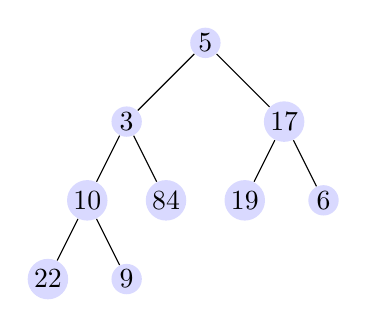
\begin{tikzpicture}[level distance=10mm] 
				\tikzstyle{every node}=[fill=blue!15,circle,inner sep=1pt] 
				\tikzstyle{level 1}=[sibling distance=20mm, 
				set style={{every node}+=[fill=blue!15]}] 
				\tikzstyle{level 2}=[sibling distance=10mm, 
				set style={{every node}+=[fill=blue!15]}] 
				\tikzstyle{level 3}=[sibling distance=10mm, 
				set style={{every node}+=[fill=blue!15]}] 
				\node {5} 
				child {node {3} 
					child {node {10} 
						child {node {22}} 
						child {node {9}} 
					} 
					child {node {84} 
					} 
				} 
				child {node {17} 
					child {node {19}  
					} 
					child {node {6}} 
				}; 
				\end{tikzpicture}
				\\
				
				\item MAX$\_$HEAPIFY(A,4):
				
				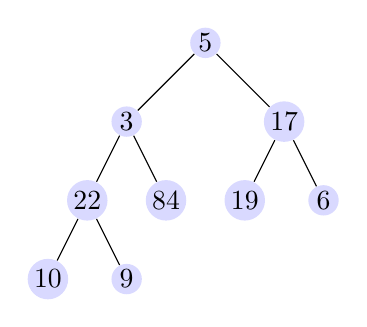
\begin{tikzpicture}[level distance=10mm] 
				\tikzstyle{every node}=[fill=blue!15,circle,inner sep=1pt] 
				\tikzstyle{level 1}=[sibling distance=20mm, 
				set style={{every node}+=[fill=blue!15]}] 
				\tikzstyle{level 2}=[sibling distance=10mm, 
				set style={{every node}+=[fill=blue!15]}] 
				\tikzstyle{level 3}=[sibling distance=10mm, 
				set style={{every node}+=[fill=blue!15]}] 
				\node {5} 
				child {node {3} 
					child {node {22} 
						child {node {10}} 
						child {node {9}} 
					} 
					child {node {84} 
					} 
				} 
				child {node {17} 
					child {node {19}  
					} 
					child {node {6}} 
				}; 
				\end{tikzpicture}
				
				\item MAX$\_$HEAPIFY(A,3):
				
				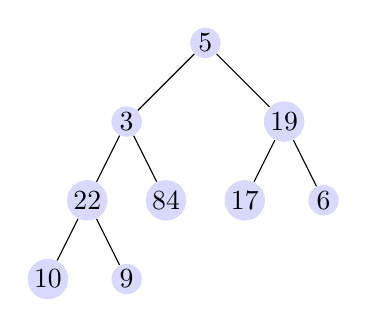
\begin{tikzpicture}[level distance=10mm] 
				\tikzstyle{every node}=[fill=blue!15,circle,inner sep=1pt] 
				\tikzstyle{level 1}=[sibling distance=20mm, 
				set style={{every node}+=[fill=blue!15]}] 
				\tikzstyle{level 2}=[sibling distance=10mm, 
				set style={{every node}+=[fill=blue!15]}] 
				\tikzstyle{level 3}=[sibling distance=10mm, 
				set style={{every node}+=[fill=blue!15]}] 
				\node {5} 
				child {node {3} 
					child {node {22} 
						child {node {10}} 
						child {node {9}} 
					} 
					child {node {84} 
					} 
				} 
				child {node {19} 
					child {node {17}  
					} 
					child {node {6}} 
				}; 
				\end{tikzpicture}
				
				\item MAX$\_$HEAPIFY(A,2):
				
				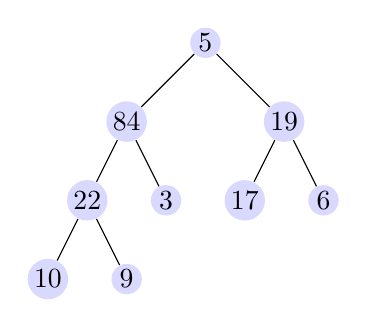
\begin{tikzpicture}[level distance=10mm] 
				\tikzstyle{every node}=[fill=blue!15,circle,inner sep=1pt] 
				\tikzstyle{level 1}=[sibling distance=20mm, 
				set style={{every node}+=[fill=blue!15]}] 
				\tikzstyle{level 2}=[sibling distance=10mm, 
				set style={{every node}+=[fill=blue!15]}] 
				\tikzstyle{level 3}=[sibling distance=10mm, 
				set style={{every node}+=[fill=blue!15]}] 
				\node {5} 
				child {node {84} 
					child {node {22} 
						child {node {10}} 
						child {node {9}} 
					} 
					child {node {3} 
					} 
				} 
				child {node {19} 
					child {node {17}  
					} 
					child {node {6}} 
				}; 
				\end{tikzpicture}
				
				\item MAX$\_$HEAPIFY(A,1):
				
				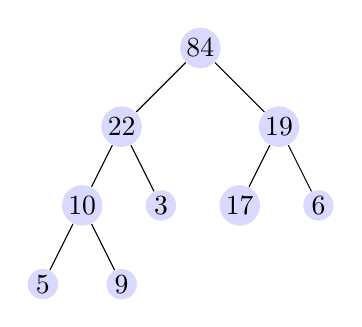
\begin{tikzpicture}[level distance=10mm] 
				\tikzstyle{every node}=[fill=blue!15,circle,inner sep=1pt] 
				\tikzstyle{level 1}=[sibling distance=20mm, 
				set style={{every node}+=[fill=blue!15]}] 
				\tikzstyle{level 2}=[sibling distance=10mm, 
				set style={{every node}+=[fill=blue!15]}] 
				\tikzstyle{level 3}=[sibling distance=10mm, 
				set style={{every node}+=[fill=blue!15]}] 
				\node {84} 
				child {node {22} 
					child {node {10} 
						child {node {5}} 
						child {node {9}} 
					} 
					child {node {3} 
					} 
				} 
				child {node {19} 
					child {node {17}  
					} 
					child {node {6}} 
				}; 
				\end{tikzpicture}
				
			\end{enumerate}
		\end{solutionorbox}
		
		\ifprintanswers
		\newpage
		\else
		\bigskip
		\fi
		
		
		%%%%%%%%%%%%%%%%%%%%%%%%%%%%%%%%%%%%%%%%%%%%%%%%%%%%%%%%%%%%%%%%%%
		%
		% Question 7
		%
		%%%%%%%%%%%%%%%%%%%%%%%%%%%%%%%%%%%%%%%%%%%%%%%%%%%%%%%%%%%%%%%%%%
		\question[5]
		6.3-2.  Why do we want the loop index $i$ in line 3 of $\proc{Build-Max-Heap}$ to decrease from $\floor{A.length/2}$ to 1 rather than increase from 1 to $\floor{A.length/2}$?
		
		\begin{solutionorbox}
			We loop index to decrease from n/2 to 1, because we need to make sure that the precondition of Max-Heapify is be met before by calling it. Every index from n/2 + 1 to n is Max-Heapified as they are all leaves. So this way after each iteration i, both left and right subtrees of node i are Max-Heapified. Instead, if we go the other way we can destruct the heap property after each iteration.
		\end{solutionorbox}
		
		\ifprintanswers
		\newpage
		\else
		\bigskip
		\fi
		
		
		%%%%%%%%%%%%%%%%%%%%%%%%%%%%%%%%%%%%%%%%%%%%%%%%%%%%%%%%%%%%%%%%%%
		%
		% Question 8
		%
		%%%%%%%%%%%%%%%%%%%%%%%%%%%%%%%%%%%%%%%%%%%%%%%%%%%%%%%%%%%%%%%%%%
		\question[5]
		6.4-1.  Using Figure 6.4 as a model, illustrate (with computer software) the operation of $\proc{Heapsort}$ on the array $A = \left< 5, 13, 2, 25, 7, 17, 20, 8, 4 \right>$.
		
		\begin{solutionorbox}
			\begin{enumerate}[label=(\roman*)]
				
				\item Build-Max-Heap(A):
				
				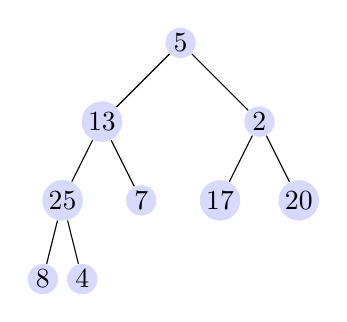
\begin{tikzpicture}[level distance=10mm] 
				\tikzstyle{every node}=[fill=blue!15,circle,inner sep=1pt] 
				\tikzstyle{level 1}=[sibling distance=20mm, 
				set style={{every node}+=[fill=blue!15]}] 
				\tikzstyle{level 2}=[sibling distance=10mm, 
				set style={{every node}+=[fill=blue!15]}] 
				\tikzstyle{level 3}=[sibling distance=5mm, 
				set style={{every node}+=[fill=blue!15]}] 
				\node {5} 
				child {node {13} 
					child {node {25} 
						child {node {8}} 
						child {node {4}} 
					} 
					child {node {7} 
					} 
				} 
				child {node {2} 
					child {node {17}  
					} 
					child {node {20}} 
				}; 
				\end{tikzpicture}
				
				\item Max-Heapify(A,4):
				
				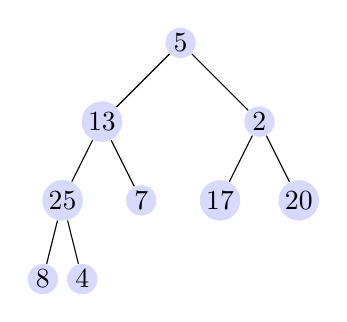
\begin{tikzpicture}[level distance=10mm] 
				\tikzstyle{every node}=[fill=blue!15,circle,inner sep=1pt] 
				\tikzstyle{level 1}=[sibling distance=20mm, 
				set style={{every node}+=[fill=blue!15]}] 
				\tikzstyle{level 2}=[sibling distance=10mm, 
				set style={{every node}+=[fill=blue!15]}] 
				\tikzstyle{level 3}=[sibling distance=5mm, 
				set style={{every node}+=[fill=blue!15]}] 
				\node {5} 
				child {node {13} 
					child {node {25} 
						child {node {8}} 
						child {node {4}} 
					} 
					child {node {7} 
					} 
				} 
				child {node {2} 
					child {node {17}  
					} 
					child {node {20}} 
				}; 
				\end{tikzpicture}
				
				\item Max-Heapify(A,3):
				
				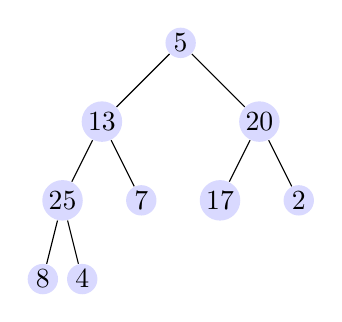
\begin{tikzpicture}[level distance=10mm] 
				\tikzstyle{every node}=[fill=blue!15,circle,inner sep=1pt] 
				\tikzstyle{level 1}=[sibling distance=20mm, 
				set style={{every node}+=[fill=blue!15]}] 
				\tikzstyle{level 2}=[sibling distance=10mm, 
				set style={{every node}+=[fill=blue!15]}] 
				\tikzstyle{level 3}=[sibling distance=5mm, 
				set style={{every node}+=[fill=blue!15]}] 
				\node {5} 
				child {node {13} 
					child {node {25} 
						child {node {8}} 
						child {node {4}} 
					} 
					child {node {7} 
					} 
				} 
				child {node {20} 
					child {node {17}  
					} 
					child {node {2}} 
				}; 
				\end{tikzpicture}
				
				\item Max-Heapify(A,2):
				
				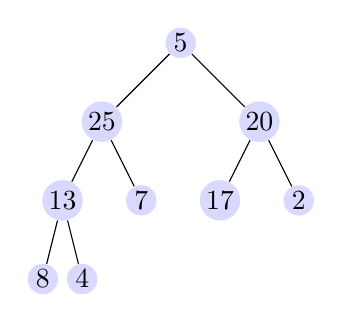
\begin{tikzpicture}[level distance=10mm] 
				\tikzstyle{every node}=[fill=blue!15,circle,inner sep=1pt] 
				\tikzstyle{level 1}=[sibling distance=20mm, 
				set style={{every node}+=[fill=blue!15]}] 
				\tikzstyle{level 2}=[sibling distance=10mm, 
				set style={{every node}+=[fill=blue!15]}] 
				\tikzstyle{level 3}=[sibling distance=5mm, 
				set style={{every node}+=[fill=blue!15]}] 
				\node {5} 
				child {node {25} 
					child {node {13} 
						child {node {8}} 
						child {node {4}} 
					} 
					child {node {7} 
					} 
				} 
				child {node {20} 
					child {node {17}  
					} 
					child {node {2}} 
				}; 
				\end{tikzpicture}
				
				\item Max-Heapify(A,1):
				
				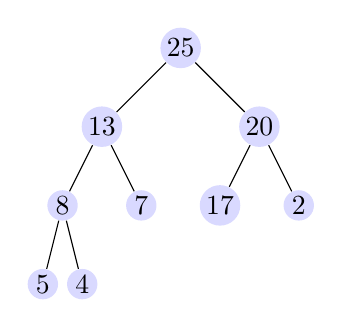
\begin{tikzpicture}[level distance=10mm] 
				\tikzstyle{every node}=[fill=blue!15,circle,inner sep=1pt] 
				\tikzstyle{level 1}=[sibling distance=20mm, 
				set style={{every node}+=[fill=blue!15]}] 
				\tikzstyle{level 2}=[sibling distance=10mm, 
				set style={{every node}+=[fill=blue!15]}] 
				\tikzstyle{level 3}=[sibling distance=5mm, 
				set style={{every node}+=[fill=blue!15]}] 
				\node {25} 
				child {node {13} 
					child {node {8} 
						child {node {5}} 
						child {node {4}} 
					} 
					child {node {7} 
					} 
				} 
				child {node {20} 
					child {node {17}  
					} 
					child {node {2}} 
				}; 
				\end{tikzpicture}\\
				
				\item Heap-Sort(A):
				
				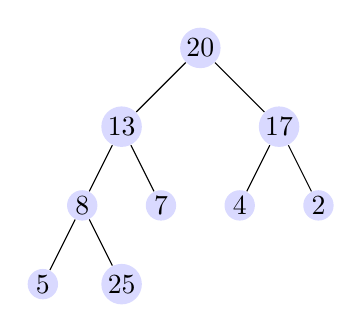
\begin{tikzpicture}[level distance=10mm] 
				\tikzstyle{every node}=[fill=blue!15,circle,inner sep=1pt] 
				\tikzstyle{level 1}=[sibling distance=20mm, 
				set style={{every node}+=[fill=blue!15]}] 
				\tikzstyle{level 2}=[sibling distance=10mm, 
				set style={{every node}+=[fill=blue!15]}] 
				\tikzstyle{level 3}=[sibling distance=10mm, 
				set style={{every node}+=[fill=blue!15]}] 
				\node {20} 
				child {node {13} 
					child {node {8} 
						child {node {5}} 
						child {node {25}} 
					} 
					child {node {7} 
					} 
				} 
				child {node {17} 
					child {node {4}  
					} 
					child {node {2}} 
				}; 
				\end{tikzpicture}
				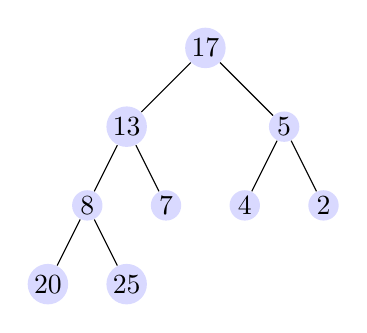
\begin{tikzpicture}[level distance=10mm] 
				\tikzstyle{every node}=[fill=blue!15,circle,inner sep=1pt] 
				\tikzstyle{level 1}=[sibling distance=20mm, 
				set style={{every node}+=[fill=blue!15]}] 
				\tikzstyle{level 2}=[sibling distance=10mm, 
				set style={{every node}+=[fill=blue!15]}] 
				\tikzstyle{level 3}=[sibling distance=10mm, 
				set style={{every node}+=[fill=blue!15]}] 
				\node {17} 
				child {node {13} 
					child {node {8} 
						child {node {20}} 
						child {node {25}} 
					} 
					child {node {7} 
					} 
				} 
				child {node {5} 
					child {node {4}  
					} 
					child {node {2}} 
				}; 
				\end{tikzpicture}
				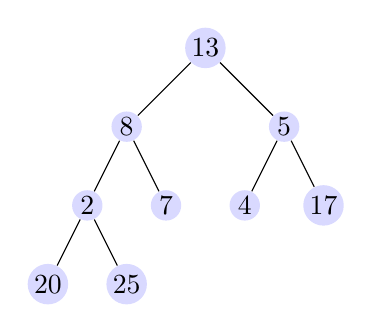
\begin{tikzpicture}[level distance=10mm] 
				\tikzstyle{every node}=[fill=blue!15,circle,inner sep=1pt] 
				\tikzstyle{level 1}=[sibling distance=20mm, 
				set style={{every node}+=[fill=blue!15]}] 
				\tikzstyle{level 2}=[sibling distance=10mm, 
				set style={{every node}+=[fill=blue!15]}] 
				\tikzstyle{level 3}=[sibling distance=10mm, 
				set style={{every node}+=[fill=blue!15]}] 
				\node {13} 
				child {node {8} 
					child {node {2} 
						child {node {20}} 
						child {node {25}} 
					} 
					child {node {7} 
					} 
				} 
				child {node {5} 
					child {node {4}  
					} 
					child {node {17}} 
				}; 
				\end{tikzpicture}\\
				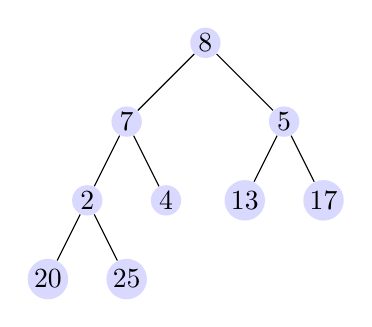
\begin{tikzpicture}[level distance=10mm] 
				\tikzstyle{every node}=[fill=blue!15,circle,inner sep=1pt] 
				\tikzstyle{level 1}=[sibling distance=20mm, 
				set style={{every node}+=[fill=blue!15]}] 
				\tikzstyle{level 2}=[sibling distance=10mm, 
				set style={{every node}+=[fill=blue!15]}] 
				\tikzstyle{level 3}=[sibling distance=10mm, 
				set style={{every node}+=[fill=blue!15]}] 
				\node {8} 
				child {node {7} 
					child {node {2} 
						child {node {20}} 
						child {node {25}} 
					} 
					child {node {4} 
					} 
				} 
				child {node {5} 
					child {node {13}  
					} 
					child {node {17}} 
				}; 
				\end{tikzpicture}
				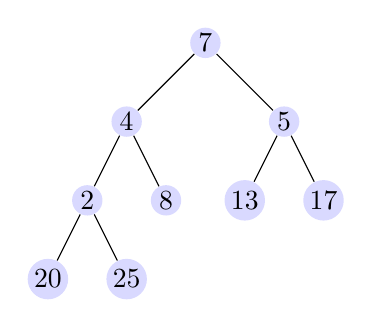
\begin{tikzpicture}[level distance=10mm] 
				\tikzstyle{every node}=[fill=blue!15,circle,inner sep=1pt] 
				\tikzstyle{level 1}=[sibling distance=20mm, 
				set style={{every node}+=[fill=blue!15]}] 
				\tikzstyle{level 2}=[sibling distance=10mm, 
				set style={{every node}+=[fill=blue!15]}] 
				\tikzstyle{level 3}=[sibling distance=10mm, 
				set style={{every node}+=[fill=blue!15]}] 
				\node {7} 
				child {node {4} 
					child {node {2} 
						child {node {20}} 
						child {node {25}} 
					} 
					child {node {8} 
					} 
				} 
				child {node {5} 
					child {node {13}  
					} 
					child {node {17}} 
				}; 
				\end{tikzpicture}
				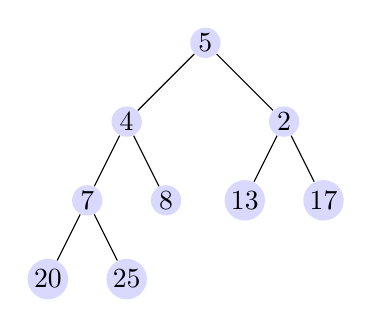
\begin{tikzpicture}[level distance=10mm] 
				\tikzstyle{every node}=[fill=blue!15,circle,inner sep=1pt] 
				\tikzstyle{level 1}=[sibling distance=20mm, 
				set style={{every node}+=[fill=blue!15]}] 
				\tikzstyle{level 2}=[sibling distance=10mm, 
				set style={{every node}+=[fill=blue!15]}] 
				\tikzstyle{level 3}=[sibling distance=10mm, 
				set style={{every node}+=[fill=blue!15]}] 
				\node {5} 
				child {node {4} 
					child {node {7} 
						child {node {20}} 
						child {node {25}} 
					} 
					child {node {8} 
					} 
				} 
				child {node {2} 
					child {node {13}  
					} 
					child {node {17}} 
				}; 
				\end{tikzpicture}\\
				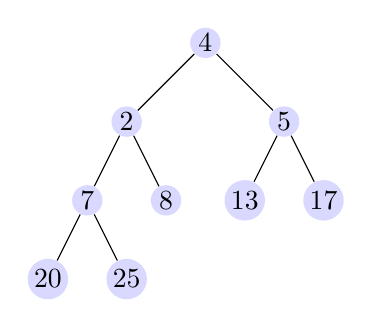
\begin{tikzpicture}[level distance=10mm] 
				\tikzstyle{every node}=[fill=blue!15,circle,inner sep=1pt] 
				\tikzstyle{level 1}=[sibling distance=20mm, 
				set style={{every node}+=[fill=blue!15]}] 
				\tikzstyle{level 2}=[sibling distance=10mm, 
				set style={{every node}+=[fill=blue!15]}] 
				\tikzstyle{level 3}=[sibling distance=10mm, 
				set style={{every node}+=[fill=blue!15]}] 
				\node {4} 
				child {node {2} 
					child {node {7} 
						child {node {20}} 
						child {node {25}} 
					} 
					child {node {8} 
					} 
				} 
				child {node {5} 
					child {node {13}  
					} 
					child {node {17}} 
				}; 
				\end{tikzpicture}
				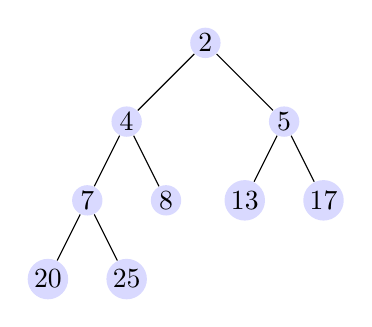
\begin{tikzpicture}[level distance=10mm] 
				\tikzstyle{every node}=[fill=blue!15,circle,inner sep=1pt] 
				\tikzstyle{level 1}=[sibling distance=20mm, 
				set style={{every node}+=[fill=blue!15]}] 
				\tikzstyle{level 2}=[sibling distance=10mm, 
				set style={{every node}+=[fill=blue!15]}] 
				\tikzstyle{level 3}=[sibling distance=10mm, 
				set style={{every node}+=[fill=blue!15]}] 
				\node {2} 
				child {node {4} 
					child {node {7} 
						child {node {20}} 
						child {node {25}} 
					} 
					child {node {8} 
					} 
				} 
				child {node {5} 
					child {node {13}  
					} 
					child {node {17}} 
				}; 
				\end{tikzpicture}
			\end{enumerate}
		\end{solutionorbox}
		
		\ifprintanswers
		\newpage
		\else
		\bigskip
		\fi
		
		
		%%%%%%%%%%%%%%%%%%%%%%%%%%%%%%%%%%%%%%%%%%%%%%%%%%%%%%%%%%%%%%%%%%
		%
		% Question 9
		%
		%%%%%%%%%%%%%%%%%%%%%%%%%%%%%%%%%%%%%%%%%%%%%%%%%%%%%%%%%%%%%%%%%%
		\question[5]
		6.4-3.  What is the running time of $\proc{Heapsort}$ on an array $A$ of length $n$ that is already sorted in increasing order?  What about decreasing order?
		
		\begin{solutionorbox}
			
			If A is sorted in increasing order, Build-Max-Heap will attain the maximum running time of $\Theta$(n). The n-1 calls  Max-Heapify(A, 1) will take at most O(log(n)) time, hence the running time of Heapsort will be $\Theta$(n lg(n)).
			
			If A is sorted in decreasing order, Build-Max-Heap will be faster by a constant factor , still  $\Theta$(n) . Here as well the n−1 calls Max-Heapify(A, 1) will take at most O(log(n)) time. Hence, the computation still remains the same and  the running time of Heapsort will be $\Theta$(n lg(n)).
			
		\end{solutionorbox}
		
		\ifprintanswers
		\newpage
		\else
		\bigskip
		\fi
		
		
		
		
		
	\end{questions}
\end{document}
